% !TeX root = ../main.tex

\chapter{Numerical model result}

\section{Flat subduction definition}


地球內部的隱沒傾角在地域上變化極大。對\emph{slab 2.0}全球模型中切出152條垂直於海溝的隱沒帶剖面(剖面位置參考自 \citealp{Hu2020}),計算深度0-150 公里、距離海溝800公里內的隱沒帶傾角,以每5度為一間隔,獲得全球隱沒帶傾角分佈圖,如圖$\ref{fig::number of tracsects}$所示,全球只有大約$13\%$的隱沒帶傾角低於$20^\circ$。然而,隱沒板塊角度變化僅是最初步的隱沒帶特徵之一,隱沒帶中的幾何形狀更能展現隱沒帶的特色。在上述的剖面中,隱沒帶以20度與40度傾角大小初步分成三類:低傾角隱沒帶、正常隱沒帶與高傾角隱沒帶。而正常隱沒帶與高傾角隱沒帶曲線具有一個典型的下凹特徵,如圖$\ref{fig::slab profile}$所示。

\begin{figure*}[ht!]
    \centering
    \includegraphics[width=4in]{chapter3_01.pdf}
    \caption{全球$152$條隱沒帶剖面傾角長條分布圖,其中綠底為隱沒剖面傾角低於$20^\circ$的剖面個數,佔整體$13\%$;粉紅底為剖面傾角介於$20^\circ-39^\circ$之間的剖面個數,佔整體$73\%$,粉藍底則為剖面傾角高於$40^\circ$的剖面個數,佔總體$14\%$。}
    \label{fig::number of tracsects}
\end{figure*}



大部分活躍的隱沒帶中,若僅考慮地表至200公里深的幾何構造,隱沒板塊的轉樞點接近海溝且下凹,並且只有一個轉樞點,如圖\ref{fig::slab profile}。在部分區域,板塊會有兩個下凹轉樞點,第一個轉樞點接近海溝且呈現平緩不明顯的下凹,第二個轉樞點在距海溝幾百公里遠處,曲率明顯、板塊下凹進入深部地幔,如圖\ref{fig::slab profile}所示,阿拉斯加、卡斯卡迪亞(Cascadia)、日本四國與新幾內亞等地區皆屬於此類。


另外在少數區域,隱沒板塊會有三個轉樞點,第一個轉樞點靠近海溝且下凹,第二個轉樞點深度較深呈現上凹,被視為是平坦隱沒的開始端,在這兩個轉樞點中隱沒板塊傾角正常。第三個轉樞點與第二個轉樞點深度相近,水平距離通常超過100公里以上,其曲率下凹的特徵代表著平坦隱沒的結束,平坦隱沒的距離與深度由第二與第三轉樞點所決定,如圖\ref{fig::slab profile}所示,智利、秘魯與墨西哥等地區屬於此類,在過去曾經被 Manea et al., 2017所討論。在本研究中,平坦隱沒被定義為具有三個轉樞點的隱沒板塊。



\citealp{barazangi1976}是最早提及平坦隱沒的研究,然而目前學界並沒有明確的平坦隱沒定義,因此過去研究較少將低傾角隱沒帶與平坦隱沒分開討論。低傾角隱沒帶分別落在阿拉斯加、卡斯卡迪亞、墨西哥以及安地斯隱沒帶上,這些低角度隱沒帶又可依隱沒板塊幾何形狀分為兩個類型:在深度150 公里以上有兩個鉸鏈點與三個鉸鏈點的隱沒板塊段,如圖$\ref{fig::slab profile}$所示。本研究將兩個鉸鏈點的隱沒段視為低傾角隱沒帶,隱沒板塊曲線上具有兩個下凹特徵,而三個鉸鏈點的隱沒段則視為平坦隱沒,隱沒板塊曲線上除了具有兩個下凹特徵外,包含在兩側鉸鏈點中有一近乎上凹段的鉸鏈點,有別於低傾角隱沒段的上下界深度落差可達50公里,其隱沒板塊在一固定深度幾乎維持水平狀態持續逾百公里以上。

\begin{figure*}[ht!]
    \centering
    \includegraphics[width=6in]{Slab_2.0_v1.pdf}
    \caption{slab 2.0 模型與四條參考剖面}
    \label{fig::slab profile}
\end{figure*}

目前世界上只有科科斯板塊(Cocos plate)隱沒帶上的墨西哥區域與納茲卡板塊(Nazca plate)隱沒帶上的秘魯與智利區域有平坦隱沒的現象,本研究主要探討這三個區域的隱沒帶。為了確保數值模型中隱沒板塊是否符合平坦隱沒定義,本研究利用數學定義判斷平坦隱沒是否存在。假設隱沒板塊為連續函數,令隱沒板塊方程式為$f(x)$, 其中$(x_{1},f(x_{1}))$, $(x_{2},f(x_{2}))$為x方向上最大的兩個反曲點(見圖$\ref{fig::flat slab definition}$)。若為平坦隱沒,需同時滿足:

1. 最大兩個反曲點水平距離需大於100公里($\mid x_{1}-x_{2}\mid > 100 km$)

2. 整段隱沒板塊斜率大於 -0.2之距離需大於50公里,該段距離稱為平坦隱沒之平坦段長度,其深度中位數稱為平坦段深度。

\begin{figure*}[ht!]
    \centering
    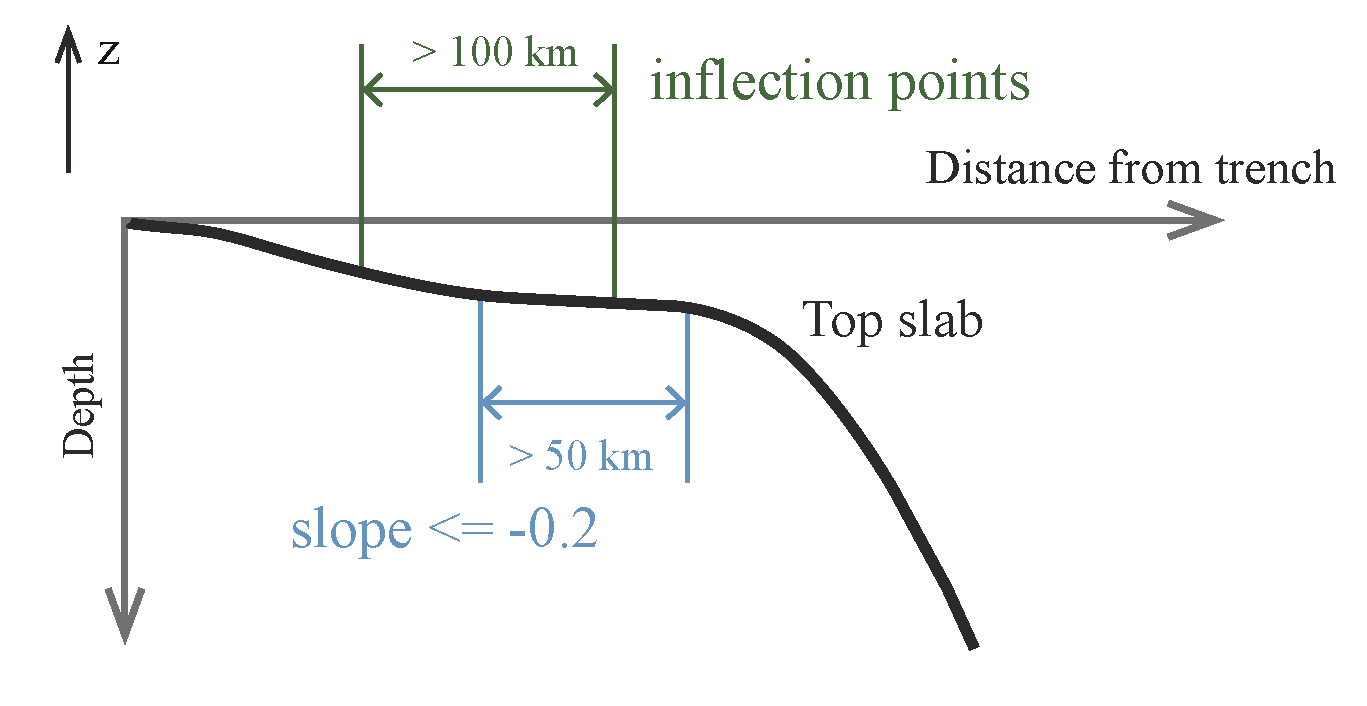
\includegraphics[width=6in]{flat_slab_definition.pdf}
    \caption{本研究中平坦隱沒的定義}
    \label{fig::flat slab definition}
\end{figure*}


比起過往研究,該數學定義更具有平坦(flat)的意義。如第一章所述,過往研究對平坦隱沒並沒有確切定義,絕大多數對平坦隱沒的判斷依據皆是以在固定深度範圍內隱沒板塊角度低於15-20度辨識為平坦隱沒,然而這種定義除了無法分辨低傾角隱沒與平坦隱沒外,所選取的隱沒板塊深度範圍是另一種可變參數,結果較為發散。

\section{Reference model of Nazca}

對於納茲卡模型,本研究建立一個長1200公里、深300公里的長方形二維剖面,包含一段長425公里的海洋岩石圈與775公里的大陸板塊,在兩個板塊交界處,建立一段長度70公里傾角50度的隱沒板塊方便後續隱沒帶發育,交接處區域的溫度較高,方便隱沒帶發育。海洋岩石圈年齡為40個百萬年(\citealp{muller2019}),包含2公里厚的沈積物、6公里厚的玄武岩與16公里厚的含水橄欖岩,熱構造由第二章提及的半空間冷卻模型決定。大陸岩石圈包含25公里厚的上部地殼與10公里厚的下部地殼,大陸岩石圈地溫梯度並沒有很好的約束,因此這裡使用地溫梯度以每公里9.5度線性遞增至140公里深(\citealp{perez2008})。由於現生地震學觀測研究提及該地區地震活動度大,且地函岩石圈速度較高、板塊脫水作用不活躍,因此納茲卡模型的蛇紋岩厚度參數設定為5公里。模型左邊界以每年5公分速率往右移動,而右邊界固定不動,符合納茲卡隱沒帶的總聚合速度。模型上邊界為自由表面,而下邊界則為開放邊界,物質可自由進出。





\section{Reference model of Cocos}


\begin{figure*}[ht!]
    \centering
    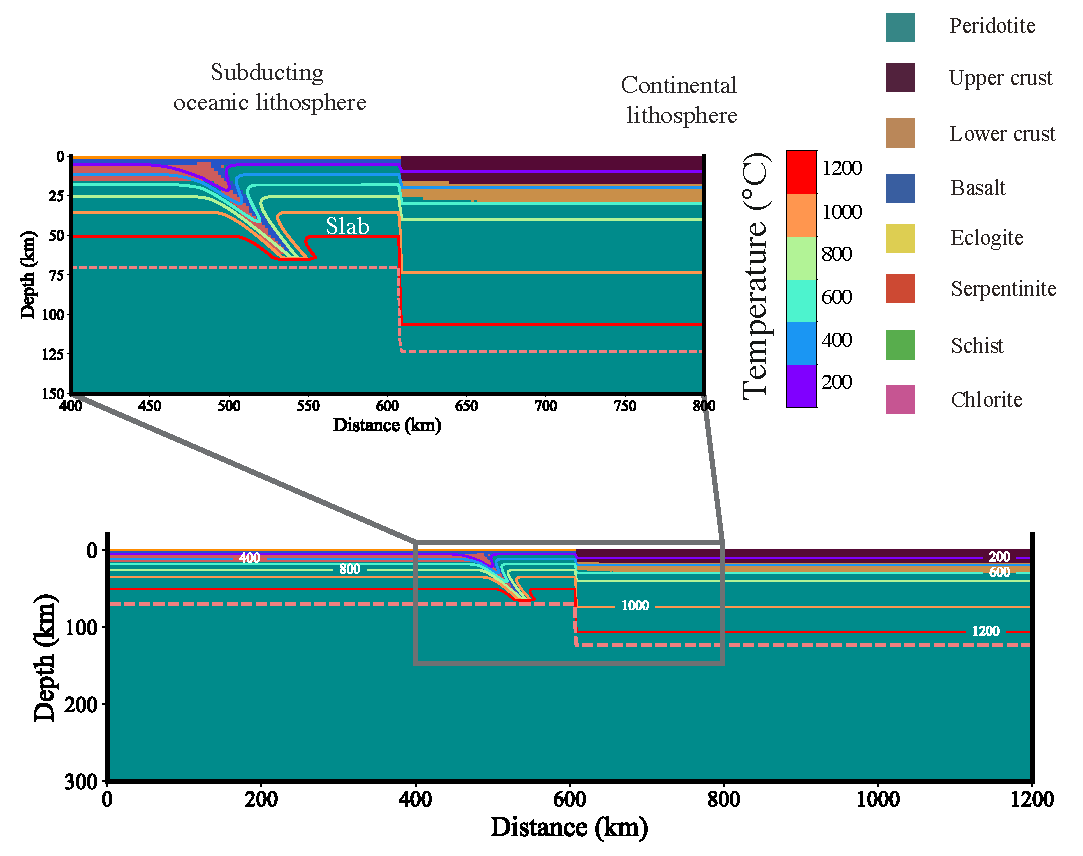
\includegraphics[width=6in]{Ref_Cocos.pdf}
    \caption{隱沒板塊模型設計與邊界條件示意圖}
    \label{fig::reference Cocos model}
\end{figure*}